\documentclass[12pt,a4paper]{article}
\usepackage[utf8]{vietnam}
\usepackage{amsmath,amssymb}
\usepackage{tabularx}
\usepackage{tikz}
\usetikzlibrary{calc,angles,quotes,arrows.meta}
\usepackage{xcolor}
\usepackage{enumitem}
\usepackage{fancyhdr}
\usepackage[top=1.0cm, bottom=1.1cm, left=1.3cm, right=1.3cm]{geometry}
\usepackage[dethi]{ex_test}
\SAOPTN{widthSA=3.2,heightSA=0.62}

\setlength{\headheight}{15pt}
\setlength{\parskip}{1.5pt}

\pagestyle{fancy}
\fancyhf{}
\lhead{\textit{Trường THCS Sơn Tây -- Đề KSCL Lớp 9 Lần 1 (2026 -- 2027)}}
\rhead{\textit{Mã đề: 01 -- Môn Toán}}
\cfoot{\thepage/2}

\begin{document}

% =============================================================================
% TRANG 1: TIÊU ĐỀ & PHẦN I TRẮC NGHIỆM
% =============================================================================
\noindent
\begin{tabularx}{\linewidth}{X r}
  \textbf{TRƯỜNG THCS SƠN TÂY} & \textbf{ĐỀ KHẢO SÁT CHẤT LƯỢNG LỚP 9 -- LẦN 1} \\
  \textbf{NĂM HỌC 2026 -- 2027} & \textbf{MÔN: TOÁN} \\
  \textbf{MÃ ĐỀ: 01} \textit{(Đề thi gồm 02 trang)} & \textit{Thời gian làm bài: 90 phút (không kể thời gian giao đề)} \\
\end{tabularx}
\vspace{-1mm}
\hrule
\vspace{2mm}

\noindent\textbf{Họ và tên thí sinh:} \dotfill \textbf{Lớp:} \dotfill \textbf{SBD:} \dotfill

\vspace{2mm}
\noindent\textbf{\large PHẦN I. TRẮC NGHIỆM KHÁCH QUAN (2,0 điểm)}

\noindent\textit{Học sinh trả lời từ Câu 1 đến Câu 8. Mỗi câu hỏi chỉ chọn một phương án đúng duy nhất và ghi chữ cái đứng trước phương án đó vào bảng trả lời bên dưới.}

\vspace{1.5mm}
\begin{center}
\renewcommand{\arraystretch}{1.25}
\begin{tabular}{|c|c|c|c|c|c|c|c|c|}
\hline
\textbf{Câu} & \textbf{1} & \textbf{2} & \textbf{3} & \textbf{4} & \textbf{5} & \textbf{6} & \textbf{7} & \textbf{8} \\
\hline
\textbf{Đáp án} & \hspace{1.1cm} & \hspace{1.1cm} & \hspace{1.1cm} & \hspace{1.1cm} & \hspace{1.1cm} & \hspace{1.1cm} & \hspace{1.1cm} & \hspace{1.1cm} \\
\hline
\end{tabular}
\end{center}
\vspace{1.5mm}

\begin{enumerate}[label=\textbf{Câu \arabic*.}, leftmargin=*, itemsep=3.5pt, parsep=0pt]
  \item Phương trình nào sau đây \textbf{không phải} là phương trình bậc nhất hai ẩn?
  \begin{flushleft}
    \begin{tabularx}{\linewidth}{X X X X}
      \textbf{A.} $2x = 0$ & 
      \textbf{B.} $2y - x = 0$ & 
      \textbf{C.} $x - 4y = -3$ & 
      \textbf{D.} $0x - 0y = -1$
    \end{tabularx}
  \end{flushleft}

  \item Cặp số $(x; y) = (4; 2)$ là nghiệm của hệ phương trình nào sau đây?
  \begin{flushleft}
    \begin{tabularx}{\linewidth}{X X X X}
      \textbf{A.} $\begin{cases} x - y = 2 \\ x - 5y = 4 \end{cases}$ & 
      \textbf{B.} $\begin{cases} x + y = 6 \\ 2x - 5y = 8 \end{cases}$ & 
      \textbf{C.} $\begin{cases} x + y = 6 \\ x - y = 2 \end{cases}$ & 
      \textbf{D.} $\begin{cases} x - y = 2 \\ 3x + 2y = 5 \end{cases}$
    \end{tabularx}
  \end{flushleft}

  \item Cho hai đường thẳng $d_1: 5x + y = 7$ và $d_2: -x - 3y = 21$. Gọi $M$ là giao điểm của hai đường thẳng $d_1$ và $d_2$. Tọa độ của điểm $M$ là
  \begin{flushleft}
    \begin{tabularx}{\linewidth}{X X X X}
      \textbf{A.} $M(-3; -8)$ & 
      \textbf{B.} $M(3; -8)$ & 
      \textbf{C.} $M(-3; 8)$ & 
      \textbf{D.} $M(3; 8)$
    \end{tabularx}
  \end{flushleft}

  \item Phương trình $(2x - 4)(3x + 6) = 0$ có tổng các nghiệm là
  \begin{flushleft}
    \begin{tabularx}{\linewidth}{X X X X}
      \textbf{A.} $2$ & 
      \textbf{B.} $-2$ & 
      \textbf{C.} $4$ & 
      \textbf{D.} $0$
    \end{tabularx}
  \end{flushleft}

  \item 
  \par\noindent
  \begin{minipage}[t]{0.78\linewidth}
    Biển báo giao thông Hình D.8 báo tốc độ tối thiểu cho xe cơ giới. Biển có hiệu lực bắt buộc các loại xe cơ giới vận hành với tốc độ không nhỏ hơn trị số ghi trên biển trong điều kiện giao thông thuận lợi và an toàn. Nếu một ô tô đi trên đường đó với vận tốc $a$ (km/h) thì $a$ phải thỏa mãn điều kiện nào trong các điều kiện sau?
    \begin{flushleft}
      \begin{tabularx}{\linewidth}{X X X X}
        \textbf{A.} $a < 60$ & 
        \textbf{B.} $a > 60$ & 
        \textbf{C.} $a \ge 60$ & 
        \textbf{D.} $a \le 60$
      \end{tabularx}
    \end{flushleft}
  \end{minipage}\hfill
  \begin{minipage}[t]{0.20\linewidth}
    \centering
    \vspace{-2mm}
    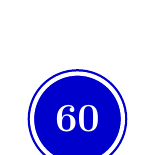
\begin{tikzpicture}[scale=0.55]
      \fill[blue!80!black] (0,0) circle (1.15);
      \draw[white, line width=1.5pt] (0,0) circle (1.05);
      \node[white, font=\bfseries\Large] at (0,0) {60};
    \end{tikzpicture}\\[1mm]
    {\scriptsize\textsf{Hình D.8 -- Biển R.306}}
  \end{minipage}

  \item Cho $\Delta ABC$ vuông tại $A$ có $AB = 3$ và $AC = 4$. Khi đó $\cos C$ bằng
  \begin{flushleft}
    \begin{tabularx}{\linewidth}{X X X X}
      \textbf{A.} $\dfrac{3}{4}$ & 
      \textbf{B.} $\dfrac{4}{3}$ & 
      \textbf{C.} $\dfrac{3}{5}$ & 
      \textbf{D.} $\dfrac{4}{5}$
    \end{tabularx}
  \end{flushleft}

  \item Cho $\Delta MNP$ vuông tại $M$ có $MN = 5\,\text{cm}$ và $NP = 10\,\text{cm}$. Khi đó số đo góc $\widehat{N} - \widehat{P}$ bằng
  \begin{flushleft}
    \begin{tabularx}{\linewidth}{X X X X}
      \textbf{A.} $60^\circ$ & 
      \textbf{B.} $30^\circ$ & 
      \textbf{C.} $90^\circ$ & 
      \textbf{D.} $45^\circ$
    \end{tabularx}
  \end{flushleft}

  \item Cho $\alpha + \beta = 90^\circ$. Khi đó giá trị của biểu thức $\sin 25^\circ + \cos 5^\circ - \cos 65^\circ - \sin 85^\circ$ bằng
  \begin{flushleft}
    \begin{tabularx}{\linewidth}{X X X X}
      \textbf{A.} $0$ & 
      \textbf{B.} $1$ & 
      \textbf{C.} $-1$ & 
      \textbf{D.} $2$
    \end{tabularx}
  \end{flushleft}
\end{enumerate}

\newpage

% =============================================================================
% TRANG 2: PHẦN II TỰ LUẬN
% =============================================================================
\noindent\textbf{\large PHẦN II. TỰ LUẬN (8,0 điểm)}

\begin{enumerate}[label=\textbf{Câu \arabic*.}, leftmargin=*, itemsep=6pt, parsep=0pt, start=9]
  \item \textbf{(2,0 điểm)} Giải các phương trình sau:
  \begin{enumerate}[label=\arabic*), leftmargin=20pt, itemsep=3pt]
    \item $(x - 4)^2 = 5x - 20$
    \item $\dfrac{1}{2x - 1} - \dfrac{3}{2x + 1} = \dfrac{6x - 3}{4x^2 - 1}$
  \end{enumerate}

  \item \textbf{(1,0 điểm)}
  \begin{enumerate}[label=\arabic*), leftmargin=20pt, itemsep=3pt]
    \item Giải bất phương trình: $\dfrac{x - 3}{5} < \dfrac{2x + 17}{3}$
    \item Cho $a < b$. Chứng minh rằng: $-3a + 2024 > -3b + 2023$.
  \end{enumerate}

  \item \textbf{(2,0 điểm)} \textit{Giải bài toán bằng cách lập hệ phương trình:}
  
  Hai ngăn của một kệ sách có tổng cộng 450 cuốn sách. Nếu chuyển 30 cuốn từ ngăn thứ nhất sang ngăn thứ hai thì số sách ở ngăn thứ nhất gấp 2 lần số sách ở ngăn thứ hai. Tính số sách ở mỗi ngăn lúc đầu?

  \item \textbf{(2,0 điểm)} 
  \par\noindent
  \begin{minipage}[t]{0.64\linewidth}
    Một người đứng ở vị trí điểm $C$ trên mặt đất cách chân tháp ăng-ten một khoảng $CD = 120\,\text{m}$. Biết rằng người ấy nhìn thấy đỉnh tháp với góc $\widehat{AOB} = 32^\circ$ so với đường nằm ngang, khoảng cách từ mắt người đó đến mặt đất là $OC = 1{,}6\,\text{m}$.
    
    Tính chiều cao $AD$ của tháp ăng-ten (kết quả làm tròn đến hai chữ số ở phần thập phân).
  \end{minipage}\hfill
  \begin{minipage}[t]{0.34\linewidth}
    \vspace{-3mm}
    \begin{center}
    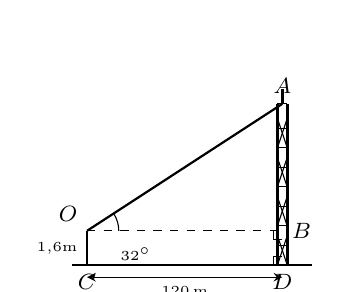
\begin{tikzpicture}[scale=0.62, >=stealth]
      \draw[thick] (-0.3,0) -- (4.6,0);
      \node[below] at (0,0) {\footnotesize $C$};
      \node[below] at (4.0,0) {\footnotesize $D$};
      
      \draw[thick] (0,0) -- (0,0.7);
      \node[above left] at (0,0.7) {\footnotesize $O$};
      \node[left] at (0,0.35) {\tiny $1{,}6\text{m}$};
      
      \coordinate (O) at (0,0.7);
      \coordinate (B) at (4.0,0.7);
      \coordinate (D) at (4.0,0);
      \coordinate (A) at (4.0,3.3);
      
      \draw[dashed] (O) -- (B);
      \node[right] at (B) {\footnotesize $B$};
      \draw[thick] (O) -- (A) node[above]{\footnotesize $A$};
      
      % Tháp AD
      \draw[line width=1.1pt] (3.9,0) -- (3.9,3.3);
      \draw[line width=1.1pt] (4.1,0) -- (4.1,3.3);
      \draw[line width=1.2pt] (4.0,3.3) -- (4.0,3.6);
      \foreach \y in {0, 0.4, 0.8, 1.2, 1.6, 2.0, 2.4, 2.8, 3.3} {
        \draw (3.9,\y) -- (4.1,\y);
      }
      \foreach \y in {0, 0.8, 1.6, 2.4} {
        \draw (3.9,\y) -- (4.1,\y+0.6);
        \draw (4.1,\y) -- (3.9,\y+0.6);
      }
      
      \draw (B) ++(0,-0.18) -- ++(-0.18,0) -- ++(0,0.18);
      \draw (D) ++(0,0.18) -- ++(-0.18,0) -- ++(0,-0.18);
      
      \draw (O) ++(0.65,0) arc (0:32:0.65);
      \node at (1.0,0.22) {\tiny $32^\circ$};
      
      \draw[<->] (0,-0.25) -- (4.0,-0.25);
      \node[below] at (2.0,-0.25) {\tiny $120\,\text{m}$};
    \end{tikzpicture}
    \end{center}
  \end{minipage}

  \item \textbf{(1,0 điểm)}
  \begin{enumerate}[label=\arabic*), leftmargin=20pt, itemsep=3pt]
    \item Giải phương trình: $\dfrac{4x}{4x^2 - 8x + 7} + \dfrac{3x}{4x^2 - 10x + 7} = 1$
    \item Cho các số $a, b, c$ dương. Chứng minh rằng:
    \[
      \frac{a}{bc} + \frac{b}{ca} + \frac{c}{ab} \ge \frac{1}{a} + \frac{1}{b} + \frac{1}{c}
    \]
  \end{enumerate}
\end{enumerate}

\vfill
\begin{center}
  \textbf{--- HẾT ---}\\
  \textit{\footnotesize Cán bộ coi thi không giải thích gì thêm.}
\end{center}

\end{document}

